\section{Branching und Merging}

\begin{frame}
  \tableofcontents[currentsection]
\end{frame}

\begin{frame}{Branching und Merging}
  \begin{figure}
    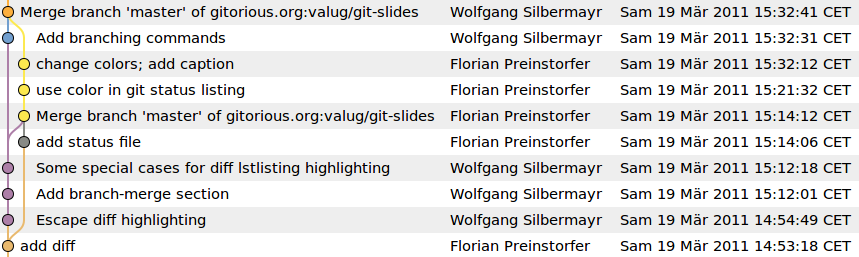
\includegraphics[width=1\textwidth]{img/branch-merge}
    \caption[format=empty]{Branching und Merging visuell dargestellt (gitg)}
  \end{figure}
\end{frame}

\begin{frame}[allowframebreaks,fragile]{Branching}
  \begin{itemize}
    \item Erzeugen von Verzweigungen
    \item Unter git sehr leichtgewichtig
    \item Jeder Branch hat einen Namen
    \item Standardmäßig wird ein \texttt{master}-Branch verwendet
    \framebreak

    \item Anzeigen aller Branches:
    \begin{lstlisting}
$ git branch
    \end{lstlisting}
    \item Anlegen eines neuen Branches:
    \begin{lstlisting}
$ git branch <branchname>
    \end{lstlisting}
    \item Wechseln auf einen anderen Branch:
    \begin{lstlisting}
$ git checkout <branchname>
    \end{lstlisting}
    \item Neuen Branch anlegen und auschecken in einem Schritt:
    \begin{lstlisting}
$ git checkout -b <branchname>
    \end{lstlisting}

  \end{itemize}

\end{frame}

\begin{frame}[allowframebreaks,fragile]{Merging}
  \begin{itemize}
    \item Zusammenführen mehrerer Branches
    \item Umfangreiche Unterstützung bei Konflikten
    \item Merging:
    \begin{lstlisting}
$ git checkout <branch>       # checkout <branch>
$ git merge <otherbranch>     # merge <otherbranch> into <branch>
$ git branch -d <otherbranch> # optionally delete <otherbranch>
    \end{lstlisting}
  \end{itemize}
\end{frame}


% vim: tabstop=2 expandtab shiftwidth=2 softtabstop=2 autoindent
